\chapter{Approche et modélisation}\label{chap:mod}
\minitoc
\e{
L'objectif de ce chapitre est de présenter notre conceptualisation et sa représentation informatique dans le cadre plus général d'une approche de description des documents audiovisuels contributive et qui suit le déroulement de la production audiovisuelle, même dans des cas de réutilisation et de production collaborative impliquant des communautés de professionnels ou d'amateurs.
Ainsi, en plus des problèmes de modélisation de la diversité des documents audiovisuels, de leur différent niveau de représentation, s'ajoute des problèmes d'échange de connaissances entre contributeurs ne partageant pas les mêmes conceptions, vocabulaires et compétences.}

\e{
Nous commençons par résumer notre analyse des langages et modélisations étudiés dans les chapitres précédents (\ref{sec:synthese}) pour mettre en évidence les manques des solutions disponibles pour répondre aux problèmes soulevés. 
Cela nous amène à présenter les principes de notre approche qui met en avant la complémentarité des informations produites avant et après la fabrication du matériel audiovisuel (\ref{sec:approche}).
Nous introduisons également l'architecture développé dans le cadre du projet MediaMap pour opérationnaliser cette approche, et notamment les applications nécessaires à son fonctionnement.
Ensuite, nous expliquons notre modélisation à travers les exemples présentés précédemment et fournissons les définitions des concepts et relations créés (\ref{sec:concept}).
Dans le chapitre \ref{chap:op}, nous discuterons la représentation de notre conceptualisation avec le langage OWL, notamment en comparant certains de nos choix avec ceux effectués dans SKOS.
Finalement, les applications développées par les partenaires du projet MediaMap et les expérimentations menées avec seront présentées plus en détails dans le chapitre \ref{chap:app}.}



\section{Synthèse de l'état de l'art}\label{sec:synthese}
Dans le chapitre \ref{chap:omod}, nous avons étudié la modélisation de connaissances par les ontologies ainsi que la modélisation des vocabulaires métiers par les terminologies. 
Notre définition des besoins implique d'associer une documentation et une terminologie à notre conceptualisation (\ref{sec:bm}), de manière à faciliter les échanges de connaissances entre tous les contributeurs de la chaîne de production, ainsi que dans les cas de réutilisation où l'on reprend des éléments externes à cette chaîne.
Nos objectifs dépassent le cadre de la modélisation documentaire que permet XML et les langages de schéma associées (\ref{sec:xml}).
Les langages de représentations des connaissances développés par le W3C apporte une formalisation qui permet de clarifier la sémantique de la modélisation et d'envisager la mise en place d'inférences (\ref{sec:onto-mc}).
Si les langages RDF et RDF-Schema permettent la définition de hiérarchies de classes et de relations, OWL ajoute de nombreux raffinements dont de nouveaux axiomes précisant l'usage des propriétés, ainsi que l'ajout de propriétés d'annotation pour décrire la conceptualisation.
La version OWL-DL fournit un compromis intéressant entre expressivité et décidabilité, mais ne permet pas de couvrir tous nos besoins [$\delta_1$ : \g{multijargon}].

Ainsi, nous avons étudié les langages de représentation de thésaurus et vocabulaire structuré (\ref{sec:thesaurus}).
SKOS et SKOS-XL proposent une représentation minimale et extensible des thésaurus existants, et apporte une formalisation qui permet leur publication sur le Web de données.
La norme ISO-25964-1 apporte la composition des termes et proposent d'associer plus d'informations sur la création, la maintenance et la documentation du thésaurus.
Les deux approches se concentrent sur la structuration des concepts auquelle on intègre (SKOS) ou on rattache des termes (dans SKOS-XL et ISO-25964-1, les termes sont définis indépendamment des concepts). 
Cependant, cette indépendance n'offre pas la possibilité de grouper les termes entre eux afin de modéliser une terminologie métier [$\delta_3$ : \g{évolution, gestion}]. 
De même, ces modèles définissent des termes préférés qui visent à normaliser l'usage linguistique d'une communauté métier, quelque soit la langue parlée par ses membres.
Les différences d'usages entre métiers, organisation ou bien entre amateur et professionnels ne sont pas représentées [$\delta_1$ : \g{multi-jargon}]. 
La documentation des concepts et des termes correspond tout à fait à nos besoins, en particulier dans SKOS avec la notion de note qui permet de s'adapter à la spécificité de chaque usage [$\delta_2$ : \g{documentation}].\\



Dans le chapitre \ref{chap:mav}, nous avons étudié la manière dont les objets audiovisuels (\ref{sec:dav}) et leur réutilisation (\ref{sec:gest}) était envisagé dans différentes communautés.
Nous avons mis en avant des divergences et des points aveugles entre les points de vue des professionnels de la production et des communautés scientifiques du multimédia, de l'ingénierie documentaire, de la sémiotique audiovisuelle et des bibliothèques numériques.
Nous nous sommes ensuite intéressés tour à tour à l'étude des formats conteneurs (\ref{sec:wrapper}) et d'autres modélisations des objets audiovisuels.

L'étude des formats conteneurs nous a montré qu'il était possible de modéliser les objets audiovisuels suivant les perspectives administratives, narratives et documentaires tout en y intégrant le matériel audiovisuel [$\chi_1$ :\g{autonomie}]. 
Cepdendant, cette forte intégration ne peut être mise en place qu'à partir de la fabrication du matériel, et en vue de son transport en fin de chaîne, et pour sa diffusion.
De même, l'utilisation d'un format conteneur façonne la modélisation autour de l'objet audiovisuel final, et même s'il embarque des métadonnées sur les fragments, elles ne peuvent être mobilisées pour elle-même.
Ainsi, la nature même du format oblitère le début de la chaîne et ne permet pas de se concentrer sur des fragments.
Par ailleurs, nous avons pointé l'ambiguïté sémantique des descriptions associées au matériel audiovisuel [$\chi_2$ :\g{réutilisabilité}].

\e{
	Les formats conteneurs ont montré l'importance de certaines informations pour le déroulement de la chaîne, et l'exploitation de document audiovisuel.
	Notre modélisation s'inspire de cette approche et vise à l'améliorer sur les aspects suivants : 
	\begin{liste}
		\item la modélisation des connaissances associées au document audiovisuel doit pouvoir débuter en début de chaîne, avant même la fabrication du matériel audiovisuel.
		\item la modélisation du document audiovisuel et des connaissances associées doit être formalisée pour éviter les ambiguïtés sémantiques ainsi que les problèmes d'appropriation de la part des contributeurs de la chaîne de production.
	\end{liste}
}

Nous avons ensuite examiné des modélisations de l'audiovisuel que l'on a distingué en deux approches, \e{endogène} et \e{exogène}, que nous jugeons complémentaires. 
Ces approches mettent l'accent respectivement sur la dimension sémiotique ou matérielle des objets audiovisuels (\ref{sec:dav}) sans vraiment les articuler.
La modélisation \e{endogène a priori} rend compte des connaissances fabriquées en début de chaîne afin de prévoir les étapes suivantes de fabrication du document et du matériel audiovisuel (\ref{sec:insitu}).
Ces modélisations se rapprochent d'une modélisation documentaire du script, définissant la structure documentaire auctoriale (\ref{sec:pv-id}) et les intentions de mise en forme.
Cette modélisation du script repose sur une unité de base qui est le plan (introduite dans ce mémoire en \ref{sec:docvoc}).
Ce découpage est particulièrement intéressant du fait que le plan est à la fois l'élément de base de la narration audiovisuelle (structure documentaire) et l'unité de travail dans le processus de production (description de la fabrication, lien avec le matériel audiovisuel). 
Il permet ainsi d'associer de multiples connaissances à des fragments audiovisuels et facilite ainsi leur réutilisation [$\chi_2$ : \g{réutilisabilité}].
Le modèle MSML se limite à une représentation XML du script utilisé pour construire une prévisualisation 3D du plateau de tournage ainsi que du résultat filmé (\ref{sec:msml}). 
Le manque de formalisation sémantique ne favorise pas la transformation de ces informations et leur association avec le matériel audiovisuel effectivement fabriqué [$\chi_1$ : \g{autonomie}].
L'autre modèle étudié propose une formalisation sémantique ainsi qu'une association entre une description du document et du matériel audiovisuel (\ref{sec:answer}).
Cependant, ces travaux ne sont pas accessibles et ne peuvent donc être repris ni évalué.

Les approches \e{exogènes} (\ref{sec:post}) proposent d'analyser le matériel audiovisuel en fin de chaîne. 
L'approche générique du schéma Dublin Core, même lorsqu'il est spécialisé pour les documents audiovisuels, est surtout pertinente au niveau du document (\ref{sec:dcmi}). 
La description des fragments n'est ainsi rendu possible que par l'utilisation de descripteurs spécifiques, comme ceux de la norme MPEG-7. 
De plus, on remarque l'importance d'une structure hiérarchique souple et extensible qui permet de couvrir les nombreux genre de documents produits par la télévision.
MPEG-7 s'est établie comme une modélisation de référence pour l'audiovisuel (\ref{sec:mpeg7}).
Pourtant, sa représentation en XML a été largement critiqué pour son ambiguïté syntaxique et sémantique qui a poussé de nombreux chercheurs à développer des formalisations sous la forme d'ontologie (\ref{sec:mpeg7etc}).
Ces modélisation sont réalisées de manière automatique ou manuelle, et certaines reposent sur une ontologie générique pour favoriser l'intégration avec des ontologies de domaines.
Au-délà de ces apports, les modèles, comme la norme originale, adopte une point de vue centré sur le matériel audiovisuel tant au niveau de la gestion que de la description des objets audiovisuels. 
Ainsi, ils négligent la modélisation de la structure documentaire et manquent de descriptions sémiotiques pertinentes pour la production audiovisuelle. % atténue l'importance de 
La gestion se fait au niveau du matériel, par identification d'une source et de variantes plus adaptées à d'autres méthodes de distribution [$\chi_1$ : \g{autonomie}].
L'abscence de distinction entre des opérations d'encodage et de montage ne permet pas de reconnaître la création d'un nouveau document (ou d'une nouvelle intention de réalisation), mais se limite à reconnaître un nouveau fichier.
De même, les descriptions sont associées aux fichiers ou bien à des entités qui représentent des ensembles de fichiers ayant des caractéristiques communes [$\chi_2$ : \g{réutilisabilité}]. 
De plus, si le découpage du matériel en segment permet de créer de multiples structure d'analyse sur l'objet, la caractérisation de ces segments par genre ne suffit pas à modéliser les contraintes de sa grammaire documentaire.
Il n'y a pas non plus de description du processus de production de ces segments, ni de l'écriture filmique.

\e{
	La production audiovisuelle et les modèles \e{endogènes} posent le plan comme l'unité de base qui structure à la fois le processus de production audiovisuelle et les échanges entre ses contributeurs, de même que les mécanismes de narration propre aux documents audiovisuels.
	La pratique de la réutilisation, les modifications et l'ouverture qu'elle engendre dans le déroulement des chaînes de production, implique également de fragmenter les documents audiovisuels, de rendre ces fragments autonomes mais aussi de les décrire pour favoriser leur circulation.
	Or la reprise des modèles existants n'est pas possible, soit par manque de formalisme sémantique, soit par manque d'accès.
	Ainsi, notre approche de modélisation doit se fonder sur le plan qui sert de point d'articulation entre une description métier, la structure documentaire et l'organisation de la production : 
	\begin{liste}
		\item la description par le vocabulaire métier de l'écriture filmique, rendu compréhensible pour les contributeurs amateurs ou externes par une terminologie et une documentation.
		\item la mise en correspondance avec d'autres niveaux de fragmentation qui constituent une structure documentaire auctoriale, régie par une grammaire de composition variable suivant le genre du document.
		\item  le processus de production qui s'organise autour des plans pour construire le document final, de la pre-script-ion, la fabrication puis le montage et autres traitements ultérieurs.
	\end{liste}
}	
\e{
	Par ailleurs, les modèles \e{exogènes} ont largement formalisé et développé la description du matériel audiovisuel par des procédés d'analyse automatique du signal.
	Si les résultats produits ne sont pas (encore) exprimés dans le vocabulaire de la production audiovisuelle, de nombreux travaux ont montré leur intérêt immédiat ainsi que les résultats potentiels pour certains types de descriptions.
	Le constat que nous faisons est que ces deux approches s'intéressent à deux moments du processus de production du document audiovisuel.
	Cela les amènent à modéliser des formes de connaissances complémentaires, utilisées à des fins différentes, que nous articulons dans une même approche de description du document audiovisuel.
	La modélisation du processus de production audiovisuelle, de ses étapes, contributeurs et produits, nous permet de réaliser cette articulation, à condition de modéliser également la forme du document en construction et d'y associer ces connaissances.
	Notre approche repose donc sur une stratégie de description du document à la fois progressive (réalisée à différents moments de la production) et contributive (réalisée par différents contributeurs, humain ou machine). 
	Il s'agit de manière concrète, de se donner des méthodes d'analyse automatique permettant de vérifier que la pre-script-ion modélisée en début de chaîne correspond au matériel effectivement fabriqué, et de la modifier si besoin afin de la transformer en description valide.
}

Enfin, nous avons également examiné une ontologie qui vise à mettre en correspondance une grande partie des modélisations de ressources multimédia sur le Web (\ref{sec:omr}).
La synthèse proposée est minimaliste et ne fait que confirmer l'impression que la plupart des modélisations attaque la modélisation des objets audiovisuels par le matériel audiovisuel (fichier et segment), plutôt que par ses aspects documentaires.
L'ontologie vise à faciliter la mise en commun des informations sur ces ressources dans le Web de données, mais ne permet pas d'étendre leur description, contrairement aux ontologies basées sur MPEG-7 et des ontologies génériques.

\e{
L'utilisation d'une ontologie générique pour intégrer des connaissances propres à d'autres domaines apparaît très au-dessus de nos besoins. 
En effet, nos ambitions se limite dans le cadre de cette thèse à l'expression des connaissances propres à la production audiovisuelle.
Ainsi, nous avons choisi de construire une ontologie noyau suivant une approche ascendante de manière à se concentrer sur les problèmes peu traités de la production audiovisuelle et éviter les écueils important de l'intégration avec une ontologie générique.}



% quelles applications pour instrumenter cette approche : introduction au chapitre 6 






% Description in situ décrivent les connaissances contenus dans le script, poussant jusqu'à instrumenter la direction du tournage ; description a posteriori se concentrent sur le signal et cherchent à créer des passerelles avec des descriptions métiers ou de domaine
% => il n'y a pas de lien entre les deux, car il n'y a pas de modélisation de la chaîne de fabrication pendant ou avant qu'elle se déroule (connaissances et produits)
% :: articuler connaissances et produits en une même modélisation dès le début de la chaîne afin de fluidifier leur circulations  
% [stratégie d'annotation pre & post fabrication du matériel]

% les formats conteneurs adoptent plusieurs perspectives sur la modélisation du contenu, mais leur représentation n'est pas formelle et comporte des ambigüités sémantiques


% Notre hypothèse est que le plan constitue l'unité signifiante de base de l'audiovisuel (FSR). C'est donc à partir d'une description de cette unité que toute description devrait commencer.
% L'indexation structurelle peut ensuite prendre place à partir de cette unité. On définit des fragments (objets éditoriaux) de niveaux supérieurs, ainsi qu'une grammaire de composition de ces fragments, ce qui permet de définir des types de documents.

% construction pendant la chaîne de production

% instrumenter l'écriture des prescriptions, structure documentaire molle, a priori qui servira également d'écriture des descriptions
% le plan est l'unité de base d'une structure documentaire qui exprime des connaissances sur la production audiovisuelle 
% ces connaissances sont adaptés à la réutilisation de contenu, puisque c'est une recherche, des opérations de réagencement qui sont fait par des contributeurs de la production, en vue d'une nouvelle production


% En toute modestie, on ne cherche pas à construire ou même à utiliser une ontologie générique, mais plutôt à se concentrer sur la modélisation de notre problème : la réutilisation dans la production audiovisuelle. Ainsi, nous ne reprennons pas directement le travail sur les ontologies génériques, car notre problème n'est pas l'intégration de connaissances d'un domaine, mais l'expression des connaissances propres à la production audiovisuelle.
% Nous nous distinguons ainsi des approches qui formalisent la modélisation de MPEG-7, car nous nous concentrons sur les connaissances fabriquées dès le début de la production. 





\section{Approche de description contributive et continue}\label{sec:approche}

\begin{cico}
\e{Comprenez-moi, mettre en machine ne signifie pas décontextualiser, mais situer autre part, dans un autre acteur, une portion des compétences nécessaires à l'action. [\dots] Au lieu de considérer des hommes d'un côté et des formalismes de l'autre, considérons plutôt une liste de compétences et cherchons expérimentalement à repérer, dans l'épreuve, lesquelles peuvent être confiées à quel genres d'acteur nouveaux.} \parcite{latour:ia}
\end{cico} 

In the context of TV production, the diversity of programs implies a diversity of workflows and editorial structures. Since a workflow specifies the asset production, it affects the collecting of information and its attachment to asset's components. Thus, distinct programs lead to distinct processes and annotation strategies. One parameter to distinguish among this diversity is the degree of shooting preparation or scripting that varies from pure scripting to pure improvisation. Between these two opposite and archetypal positions lies a variety of use-case that need to be covered. However, two kinds of program and production can be defined based on their attitude towards scripting:

\begin{itemize}
	\item[$\bullet$] on the one hand, a pure \textbf{fiction program} such as a drama, comedy, animated series etc. create original materials\footnote{Video Mash-Ups are an exception to fiction program as they rely on material editing or dubbing over existing materials to create a new storyline. For instance, \gui{Le grand Détournement} (1993 -- Michel Hazanavicius and Dominique Mézerette) which incorporates materials from over 50 movies and uses the official French dubber of John Wayne, a key character in the plot.} to tell a story and convey a message. Their major feature is that they do not need to rely on actual events to create content. In fiction, events, characters, location are created to fit the need of the story. However, these liberty comes with a challenge, convinces the viewer of the story consistency. In addition, audiovisual material creation is very expensive as it involves many equipments and people. 

Because of this control on the future content and the cost of content production, fiction tends to be planned and described as much as possible. Pre-production documents such as the shooting script can specify the editorial, structural and aesthetic outline of the content in details. As the production is contributive, these documents need to be understood by various people and thus a common language of the filmmaking has emerged. We call it the audiovisual scripting vocabulary in reference to the main document using it. This vocabulary is widely known in the professional community and can be easily learned by enthusiastic amateurs. Despite its intensive use during the production chain, it is not used later during the archiving process. 
%When modifications arise, either due to external constraints or voluntary decision, these documents are updated in order to remain a reference for all production contributors.   

	\item[$\bullet$] on the other hand, a \textbf{reality-based program} such as news, documentary, magazine, talk-show etc. aim at depicting reality and reporting it to the viewer. These programs usually rely on the recording of an event more or less expected and more or less under control. From their recordings, the program is built according to editorial guidelines that defines perspective on reality.
	
In most cases, information about the future event are known beforehand which gives the opportunity for anticipation. For instance, studio production like a game show can rely on a predefined environment with fixed positions for people, lightning, cameras etc. For documentary, the main storyline is predefined and the shooting location can be more or less controlled. In worst case, the shooting occurs without prior planning to capture an unexpected and fleeting event. Compared to fiction program, the integration of diverse and existing materials is much easier as it can be decided later in the process without putting the report's consistency in jeopardy. Moreover, as the audiovisual material creation is costly such content integration and repurposing is much favored. Yet, content description is scarce due to production time constraints and do not provide as detailed information as pre-production documents. 
\end{itemize}


\begin{figure}[ht!]
\centering
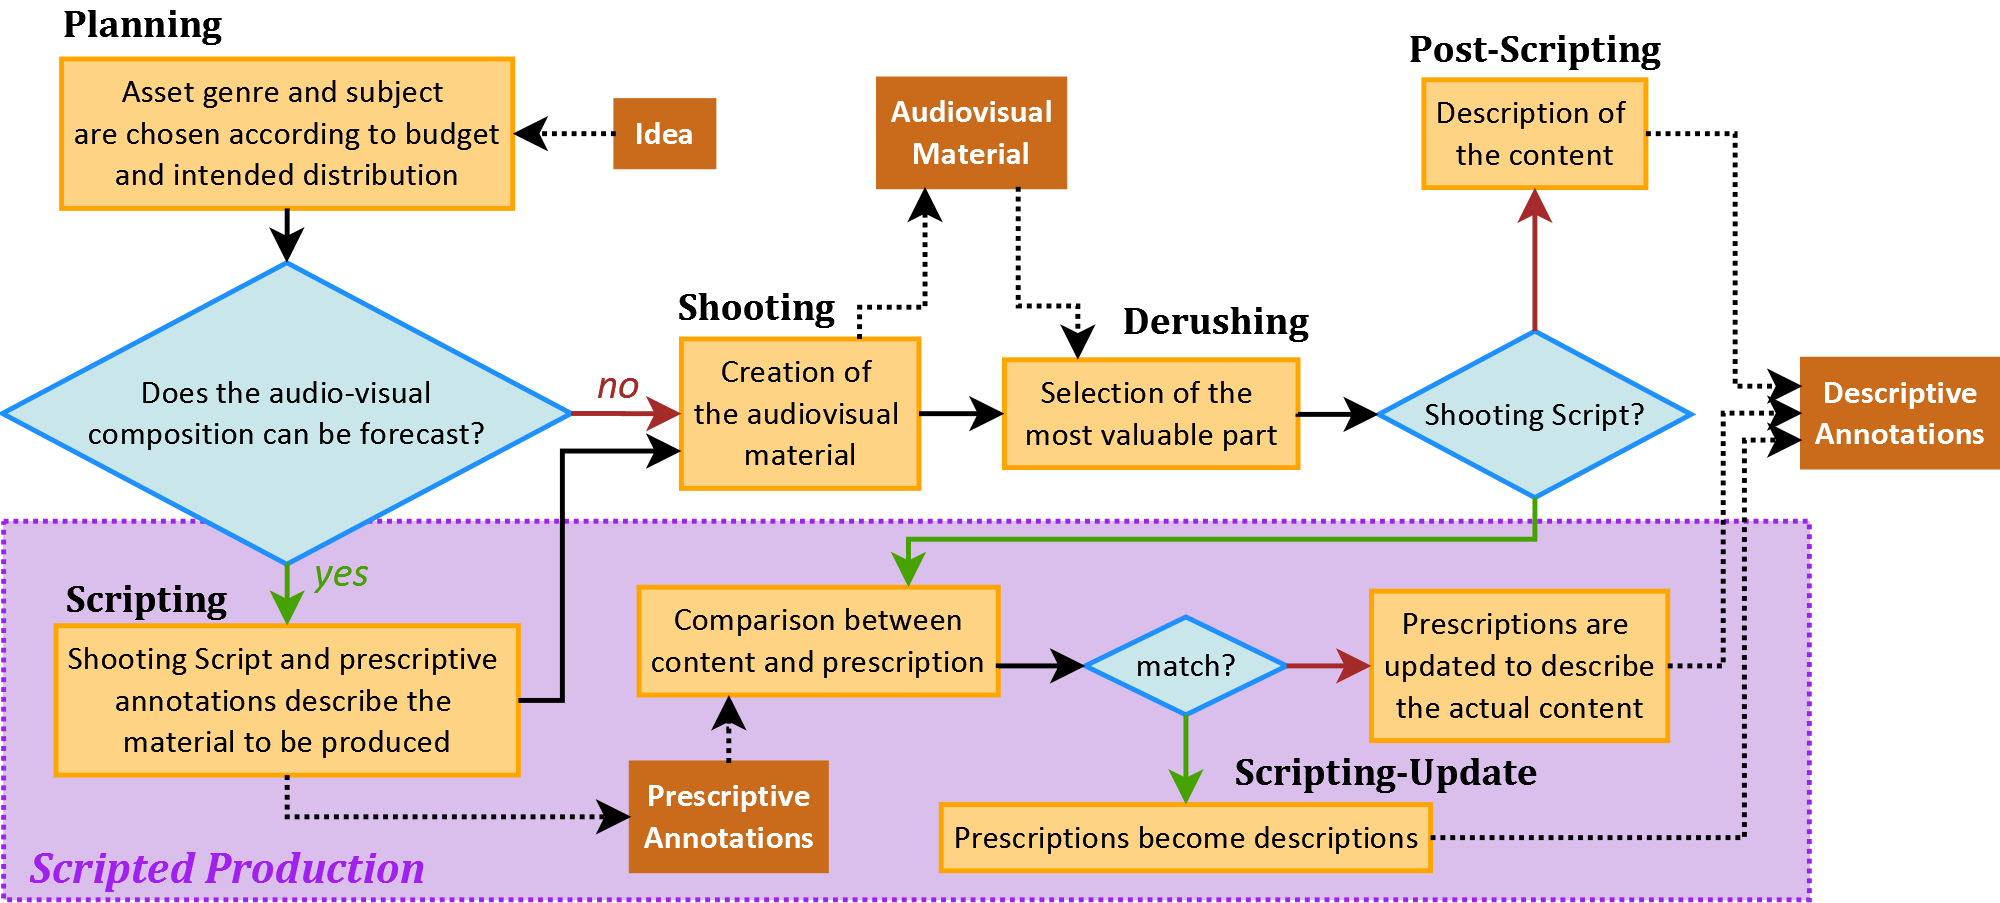
\includegraphics[width=0.9\textwidth]{./images/Approach-Logigram-v2.png}
\caption{Description continue pour des productions scriptées et non-scriptées}
\label{img:strat-annot}
\end{figure}

he modeling of the audiovisual scripting vocabulary brings potential benefits for both kinds of production. Provided that we adopt an adequate annotation strategy to collect information at various steps of the production chain. The goal is to enable audiovisual components description before, during or after their production, when the information is created or modified. The \textbf{annotation process} differences between scripted and non-scripted production are presented in Figure \ref{fig:strat-annot}.
%By modeling the audiovisual scripting vocabulary to annotate asset's content, we create a correspondence between annotations and pre-production documents. This connection can be used by a software to create and update both at the same time all along the production process. For reality-based programs, annotations can also be created later in the process. 
%The processes description will be detailed in the next section. For now on, we focus on the \textbf{annotation strategies} differences. 
At first, audiovisual production starts from an original or existing program's idea. When the idea is shaped to fit a program genre, the structure of the audiovisual document is almost fixed. In the case of scripted production, the collect of information begins with the work on pre-production documents and prescriptive annotations. Then, the audiovisual material is produced during the shooting. At the derushing stage, a selection of the best material is made depending on the intended message to convey. If prescriptive annotations have been created, they can be used as a groundwork and compared to the actual selected content. If the comparison matches, then the prescriptive annotation becomes descriptive annotations. Otherwise, the prescriptive annotations should be corrected before being accepted as descriptive annotations. For non-scripted production, the content's description really begins during the derushing stage. Finally, the output is a piece of annotated audiovisual content.

Note that these annotation strategies do not assume anything on the nature of the agent in charge of creating, checking and updating the annotations. In our mind, humans and systems have distinct capabilities which should be used in conjunction. We call this approach a \textit{continuous} (all along the production process) and \textit{contributive} (by various people or systems) description of audiovisual documents.
